\documentclass[a4paper,12pt]{article}
	
\usepackage[T2A]{fontenc}			
\usepackage[utf8]{inputenc}			
\usepackage[english,russian]{babel}	

\usepackage[
bookmarks=true, colorlinks=true, unicode=true,
urlcolor=black,linkcolor=black, anchorcolor=black,
citecolor=black, menucolor=black, filecolor=black,
]{hyperref}

\usepackage{color}
\usepackage{caption}
\DeclareCaptionFont{white}{\color{black}}
\DeclareCaptionFormat{listing}{\colorbox{white}{\parbox{\textwidth}{#1#2#3}}}
\captionsetup[lstlisting]{format=listing,labelfont=white,textfont=white}

\usepackage{amsmath,amsfonts,amssymb,amsthm,mathtools} 
\usepackage{wasysym}

\usepackage{graphicx}
%\usepackage[cache=false]{minted}
\usepackage{cmap}
\usepackage{indentfirst}

\usepackage{listings} 
\usepackage{fancyvrb}

\usepackage{geometry}
\geometry{left=2cm}
\geometry{right=1.5cm}
\geometry{top=1cm}
\geometry{bottom=2cm}

\setlength{\parindent}{5ex}
\setlength{\parskip}{0.5em}


\begin{document}
\lstset{ %
language=C++,                 % выбор языка для подсветки (здесь это С)
basicstyle=\small\sffamily, % размер и начертание шрифта для подсветки кода
numbers=left,               % где поставить нумерацию строк (слева\справа)
numberstyle=\tiny,           % размер шрифта для номеров строк
stepnumber=1,                   % размер шага между двумя номерами строк
numbersep=5pt,                % как далеко отстоят номера строк от подсвечиваемого кода
backgroundcolor=\color{white}, % цвет фона подсветки - используем \usepackage{color}
showspaces=false,            % показывать или нет пробелы специальными отступами
showstringspaces=false,      % показывать или нет пробелы в строках
showtabs=false,             % показывать или нет табуляцию в строках
frame=single,              % рисовать рамку вокруг кода
tabsize=2,                 % размер табуляции по умолчанию равен 2 пробелам
captionpos=t,              % позиция заголовка вверху [t] или внизу [b] 
breaklines=true,           % автоматически переносить строки (да\нет)
breakatwhitespace=false, % переносить строки только если есть пробел
escapeinside={\%*}{*)}   % если нужно добавить комментарии в коде
}


% Титульный лист
\large
\begin{center}
Федеральное государственное бюджетное образовательное учреждение 
высшего образования <<Московский государственный технический 
университет имени Н. Э. Баумана>> 
(национальный исследовательский университет)
\end{center}

\vspace*{30mm} 

\LARGE
\begin{center}
Дисциплина: <<Анализ алгоритмов>>

Отчет по лабораторной работе №7
\end{center}

\vspace*{30mm} 

\huge
\begin{center}
Тема работы:\\
<<Алгоритмы поиска подстроки в строке>>
\end{center}
\vspace*{30mm} 

\large
\begin{flushright}
Студент: Волков Е. А. \\
Группа: ИУ7-55Б \\
Преподаватели: Волкова Л. Л., \\ Строганов Ю. В. \\
\end{flushright}

\vspace*{40mm}
\begin{center}
Москва, 2019 г.  
\end{center}
\thispagestyle{empty}

\tableofcontents
% \setcounter{page}{1}

\section*{Введение}
\addcontentsline{toc}{section}{Введение}

\textbf{Поиск подстроки в строке} --- важная задача поиска информации.
Применяется в виде встроенной функции в текстовых редакторах, СУБД,
поисковых машинах и языках программирования.

Такой поиск приходится проводить довольно часто, поэтому необходимо, чтобы
он осуществлялся как можно быстрее. Становится ясно, что наивный алгоритм с
полным перебором всех частей строки, длины которых соответствуют
длине шаблона, является не самым эффективным способом решения такой задачи.

Существует немалое количество алгоритмов, справляющихся с поиском подстроки,
лучше, чем примитивный перебор. 

\textbf{Цель лабораторной работы:} изучение метода динамического программирования
на материале алгоритмов поиска подстроки в строке.

\textbf{Задачи работы:}
	
\begin{enumerate} 
\item[1)] изучить алгоритмы поиска подстроки в строке Кнута-Морриса-Пратта
и Бойера-Мура;
\item[2)] применить метод динамического программирования для  
реализации указанных алгоритмов;
\item[3)] провести сравнительный анализ алгоритмов по времени выполнения;
\item[4)] экспериментально подтвердить различия во временнóй эффективности алгоритмов 
при помощи разработанного программного обеспечения на материале замеров процессорного 
времени на строках различных размеров;
\item[5)] описать и обосновать полученные результаты в отчете о лабораторной 
работе, выполненного как расчётно-пояснительная записка. 
\end{enumerate} 
\pagebreak

\newpage
\section{Аналитический раздел}
	
В данном разделе будут рассмотрены выбранные алгоритмы поиска подстроки в строке.
	
\subsection{Описание алгоритмов}

\subsubsection{Алгоритм Кнута-Морриса-Пратта}

Алгоритм Кнута-Морриса-Пратта основан на принципе конечного автомата.
В этом алгоритме состояния помечаются символами, совпадение с которыми должно в данный момент произойти.
Из каждого состояния имеется два перехода: один соответствует успешному сравнению, другой — несовпадению.
Успешное сравнение переводит нас в следующий узел автомата, а в случае несовпадения мы попадаем
в предыдущий узел, отвечающий образцу.
Пример автомата Кнута-Морриса-Пратта для подстроки \textit{ababcb} приведен на рис. \ref{fig:kmp_example}. ~\cite{mcconell}

\begin{figure}[h!]
\begin{center}
{\includegraphics[scale = 0.5]{img/kmp_example.png}}
\caption{
Полный автомат Кнута-Морриса-Пратта для подстроки \textit{ababcb}}
\label{fig:kmp_example}
\end{center}
\end{figure}

При всяком переходе по успешному сравнению в конечном автомате
Кнута-Морриса-Пратта происходит выборка нового символа из текста.
Переходы, отвечающие неудачному сравнению, не приводят к выборке нового символа;
вместо этого они повторно используют последний выбранный символ. Если мы перешли в конечное состояние,
то это означает, что искомая подстрока найдена.

\subsubsection{Алгоритм Бойера-Мура}

Алгоритм Бойера-Мура осуществляет сравнение с образцом справа налево,
а не слева направо, как алгоритм Кнута-Морриса-Пратта.
Исследуя искомый образец, можно осуществлять более эффективные прыжки в тексте при обнаружении несовпадения. ~\cite{mcconell}

Рассмотрим строку \textit{there they are} и подстроку \textit{they}.
Здесь сначала сравнивается \textit{y} с \textit{r} и обнаруживается несовпадение.
Поскольку известно, что буква \textit{r} вообще не входит в образец,
можно сдвинуться в тексте на целых четыре буквы (т. е. на длину образца)
вправо. Затем сравнивается буква \textit{y} с \textit{h} и вновь обнаруживается
несовпадение. Однако поскольку на этот раз \textit{р} входит в образец,
есть возможность сдвинуться вправо только на две буквы так, чтобы буквы
\textit{h} совпали.
Затем начинается сравнение справа и обнаруживается полное совпадение кусочка текста с 
образцом. В алгоритме Бойера—Мура делается 6
сравнений вместо 13 сравнений в примитивном алгоритме, в котором
рассматриваются все подстроки исходной строки, совпадающие по длине
с шаблоном.

Пример проиллюстрирован в таблице \ref{bm_example}.

\begin{table} [h!]
\begin{center}
\caption{Поиск образца they в тексте \textit{there they are}}
\begin{tabular}{r|rrrrrrrrrrrrrr|}

           &          t &          h &          e &          r &          e &            &          t &          h &          e &          y &            &          a &          r &          e \\

         1 &          t &          h &          e &          y &            &            &            &            &            &            &            &            &            &            \\

         2 &            &            &            &            &          t &          h &          e &          y &            &            &            &            &            &            \\

         3 &            &            &            &            &            &            &          t &          h &          e &          y &            &            &            &            \\

\end{tabular}

\label{bm_example}
\end{center}
\end{table} 

Алгоритм Бойера-Мура обрабатывает образец двумя способами.
Во-первых, можно вычислить величину возможного сдвига при несовпадении
очередного символа.
Во-вторых, вычисляется величина
прыжка. Эти действия помогают эффективно подстраивать шаблон под новую подстроку.

\subsection*{Выводы}
\addcontentsline{toc}{subsection}{Выводы}

Рассмотрены алгоритмы поиска подстроки в строке,
предоставляющие, очевидно, более эффективное решение в сравнении с наивным алгоритмом.
Обоснованы различия между приведенными алгоритмами и выделены ключевые моменты
каждого из них.

\newpage
\section{Конструкторский раздел}

В разделе приводятся схемы алгоритмов Кнута-Морриса-Пратта и Бойера-Мура, приводятся примеры работы алгоритмов и производится их теоретический сравнительный анализ.

\subsection{Разработка алгоритмов}

На рис. \ref{fig:shift}-\ref{fig:bm} приведены схемы 
алгоритмов поиска подстроки.

\begin{figure}[h!]
\begin{center}
{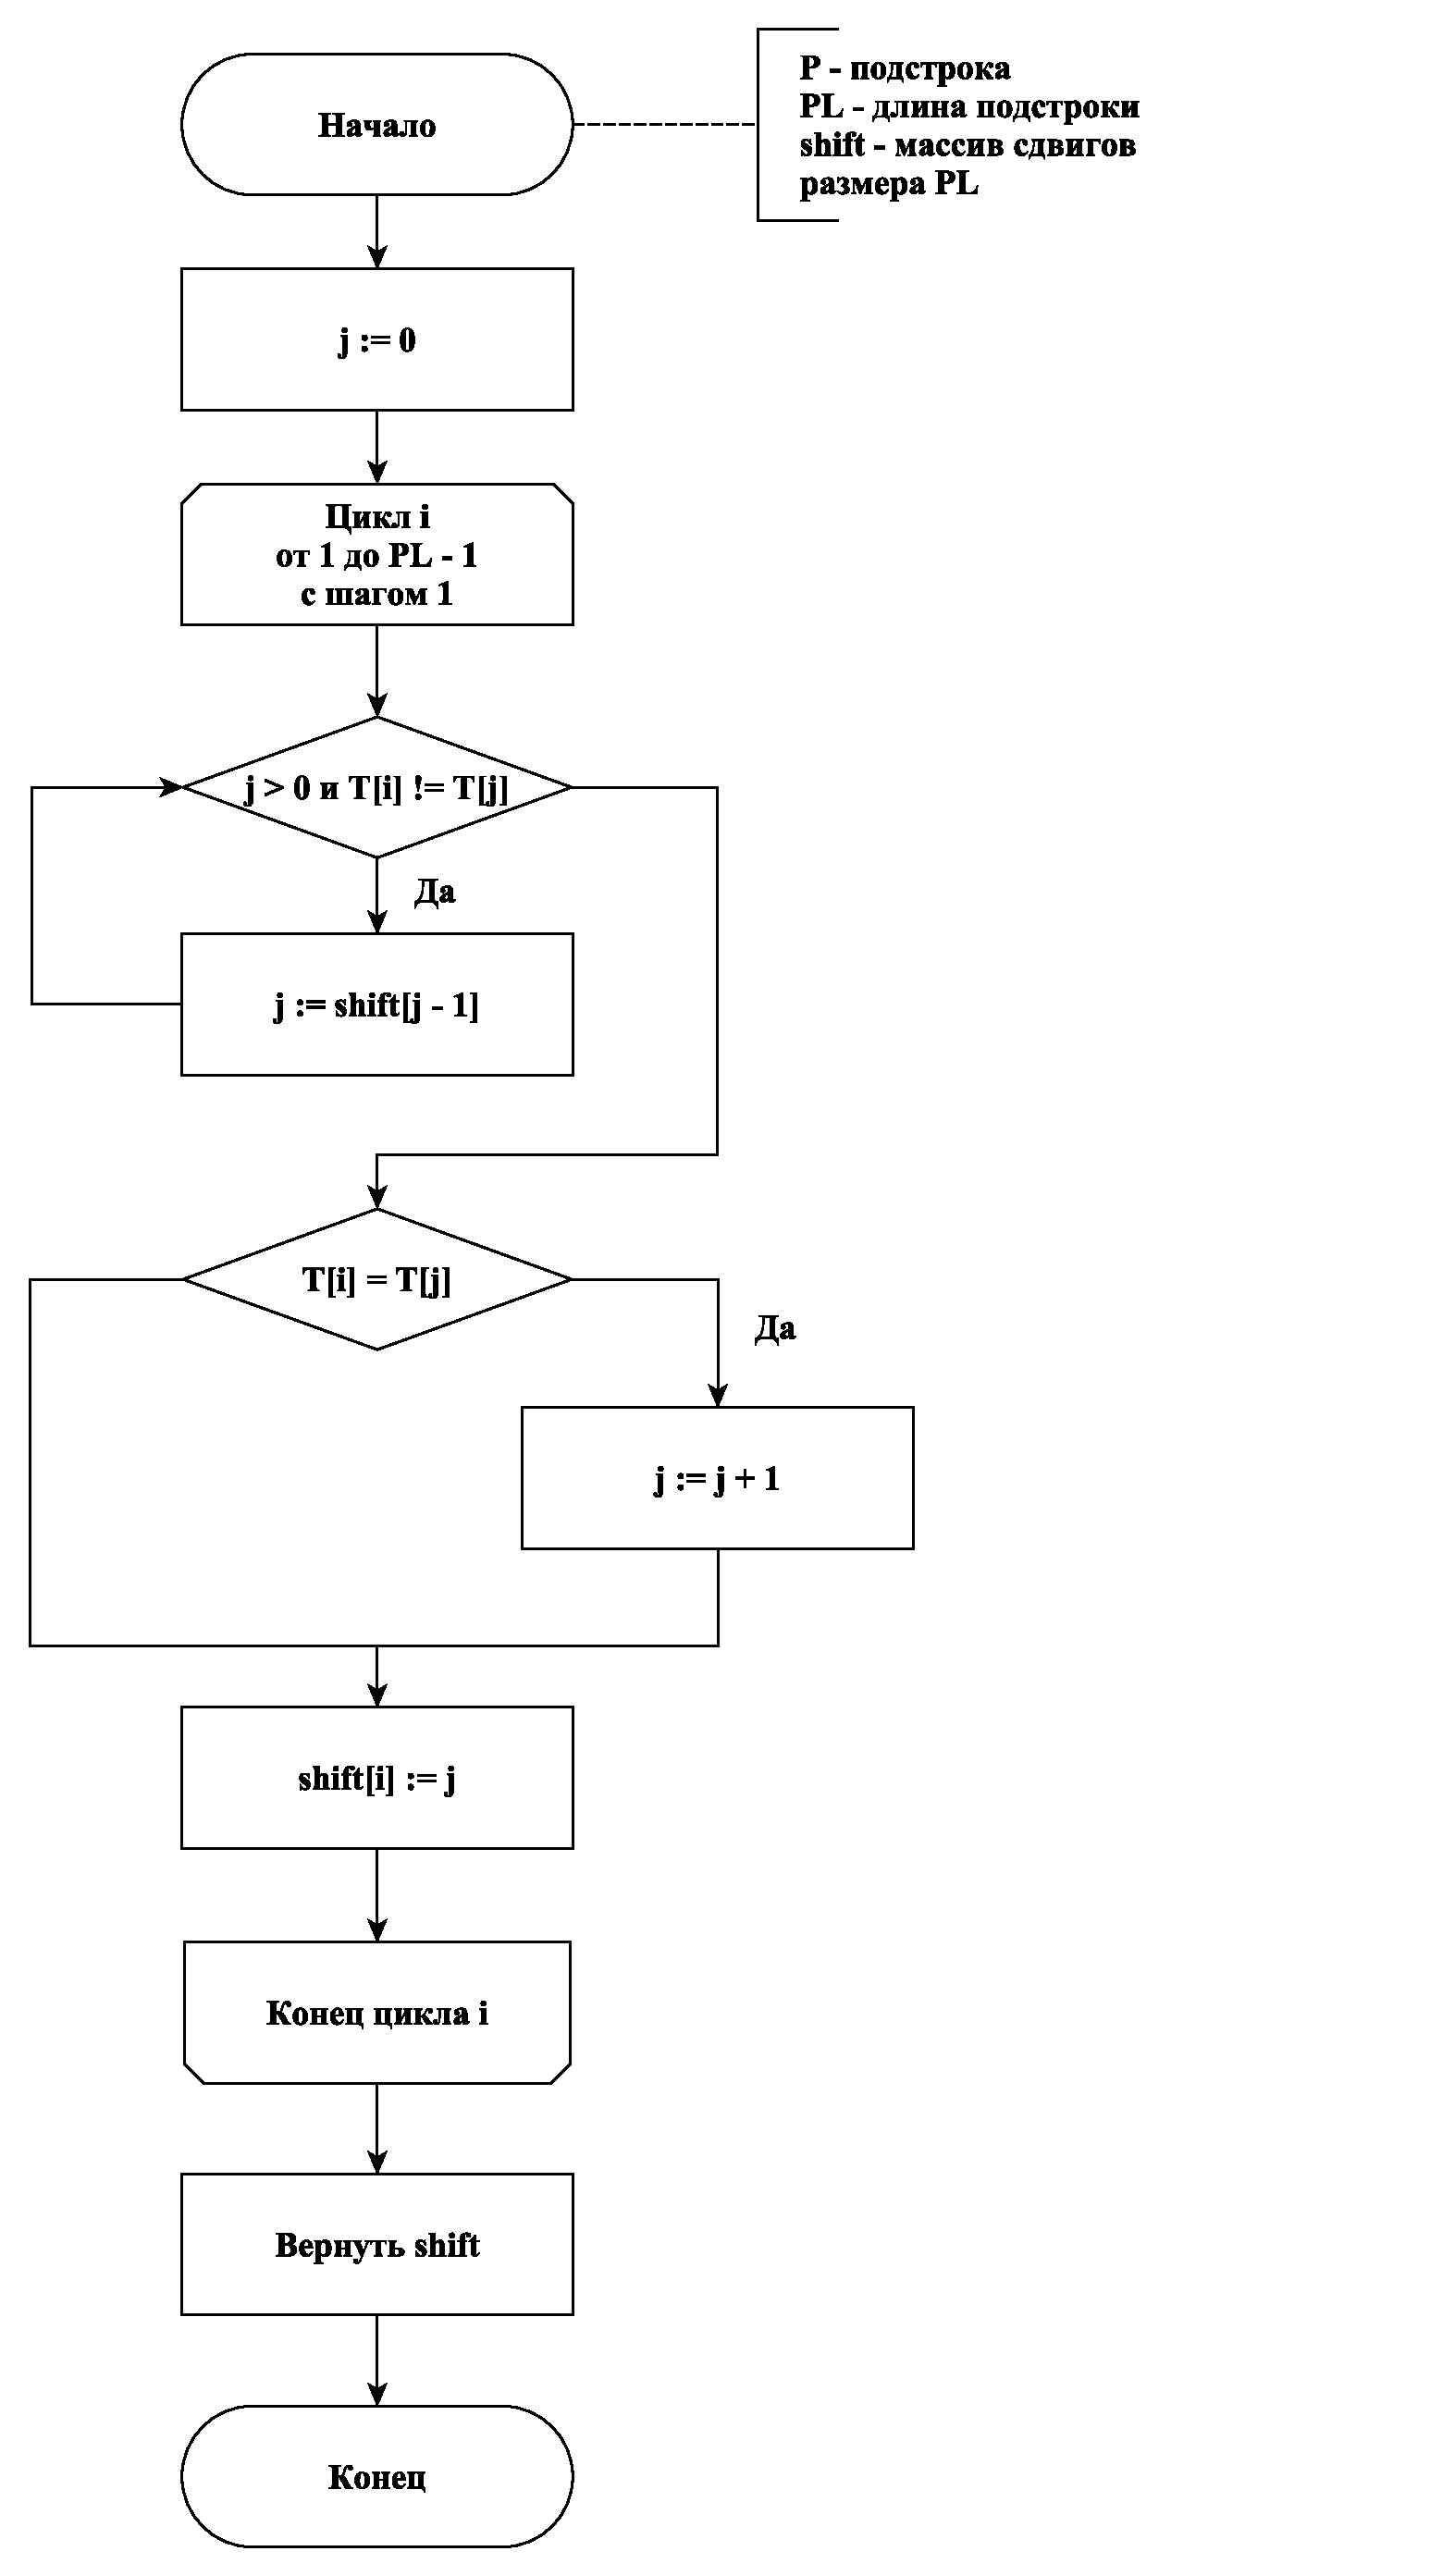
\includegraphics[scale = 0.4]{diagram/shift.pdf}}
\caption{
Схема алгоритма заполнения массива сдвигов}
\label{fig:shift}
\end{center}
\end{figure}

\pagebreak

\begin{figure}[h!]
\begin{center}
{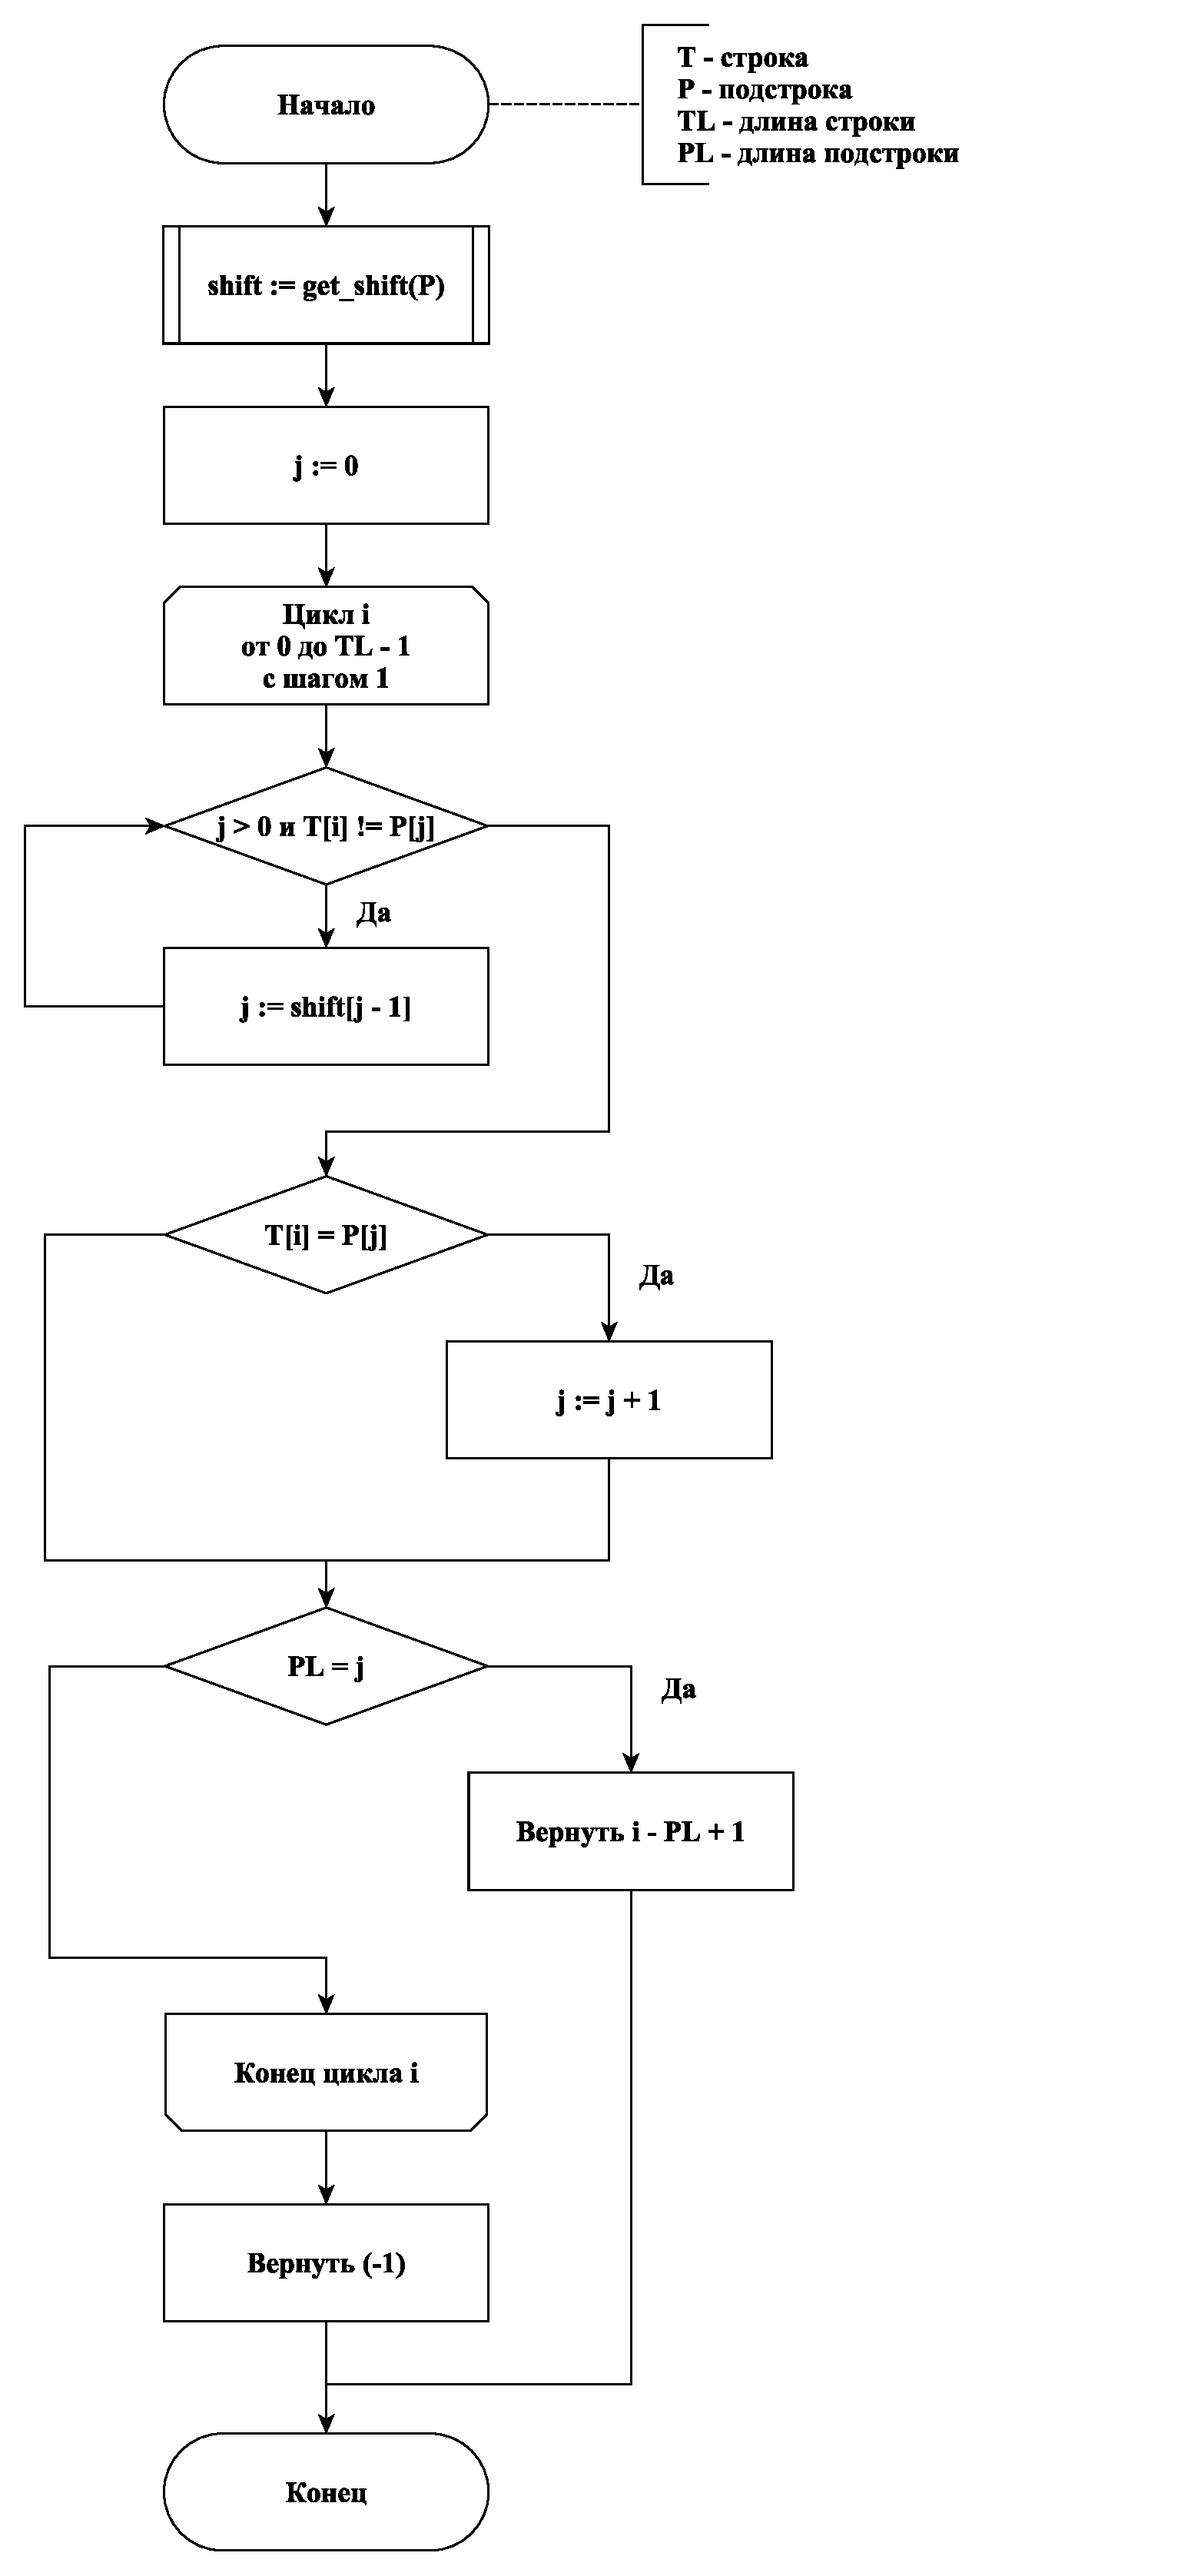
\includegraphics[scale = 0.4]{diagram/kmp.pdf}}
\caption{
Схема алгоритма Кнута-Морриса-Пратта}
\label{fig:kmp}
\end{center}
\end{figure}

\pagebreak

\begin{figure}[h!]
\begin{center}
{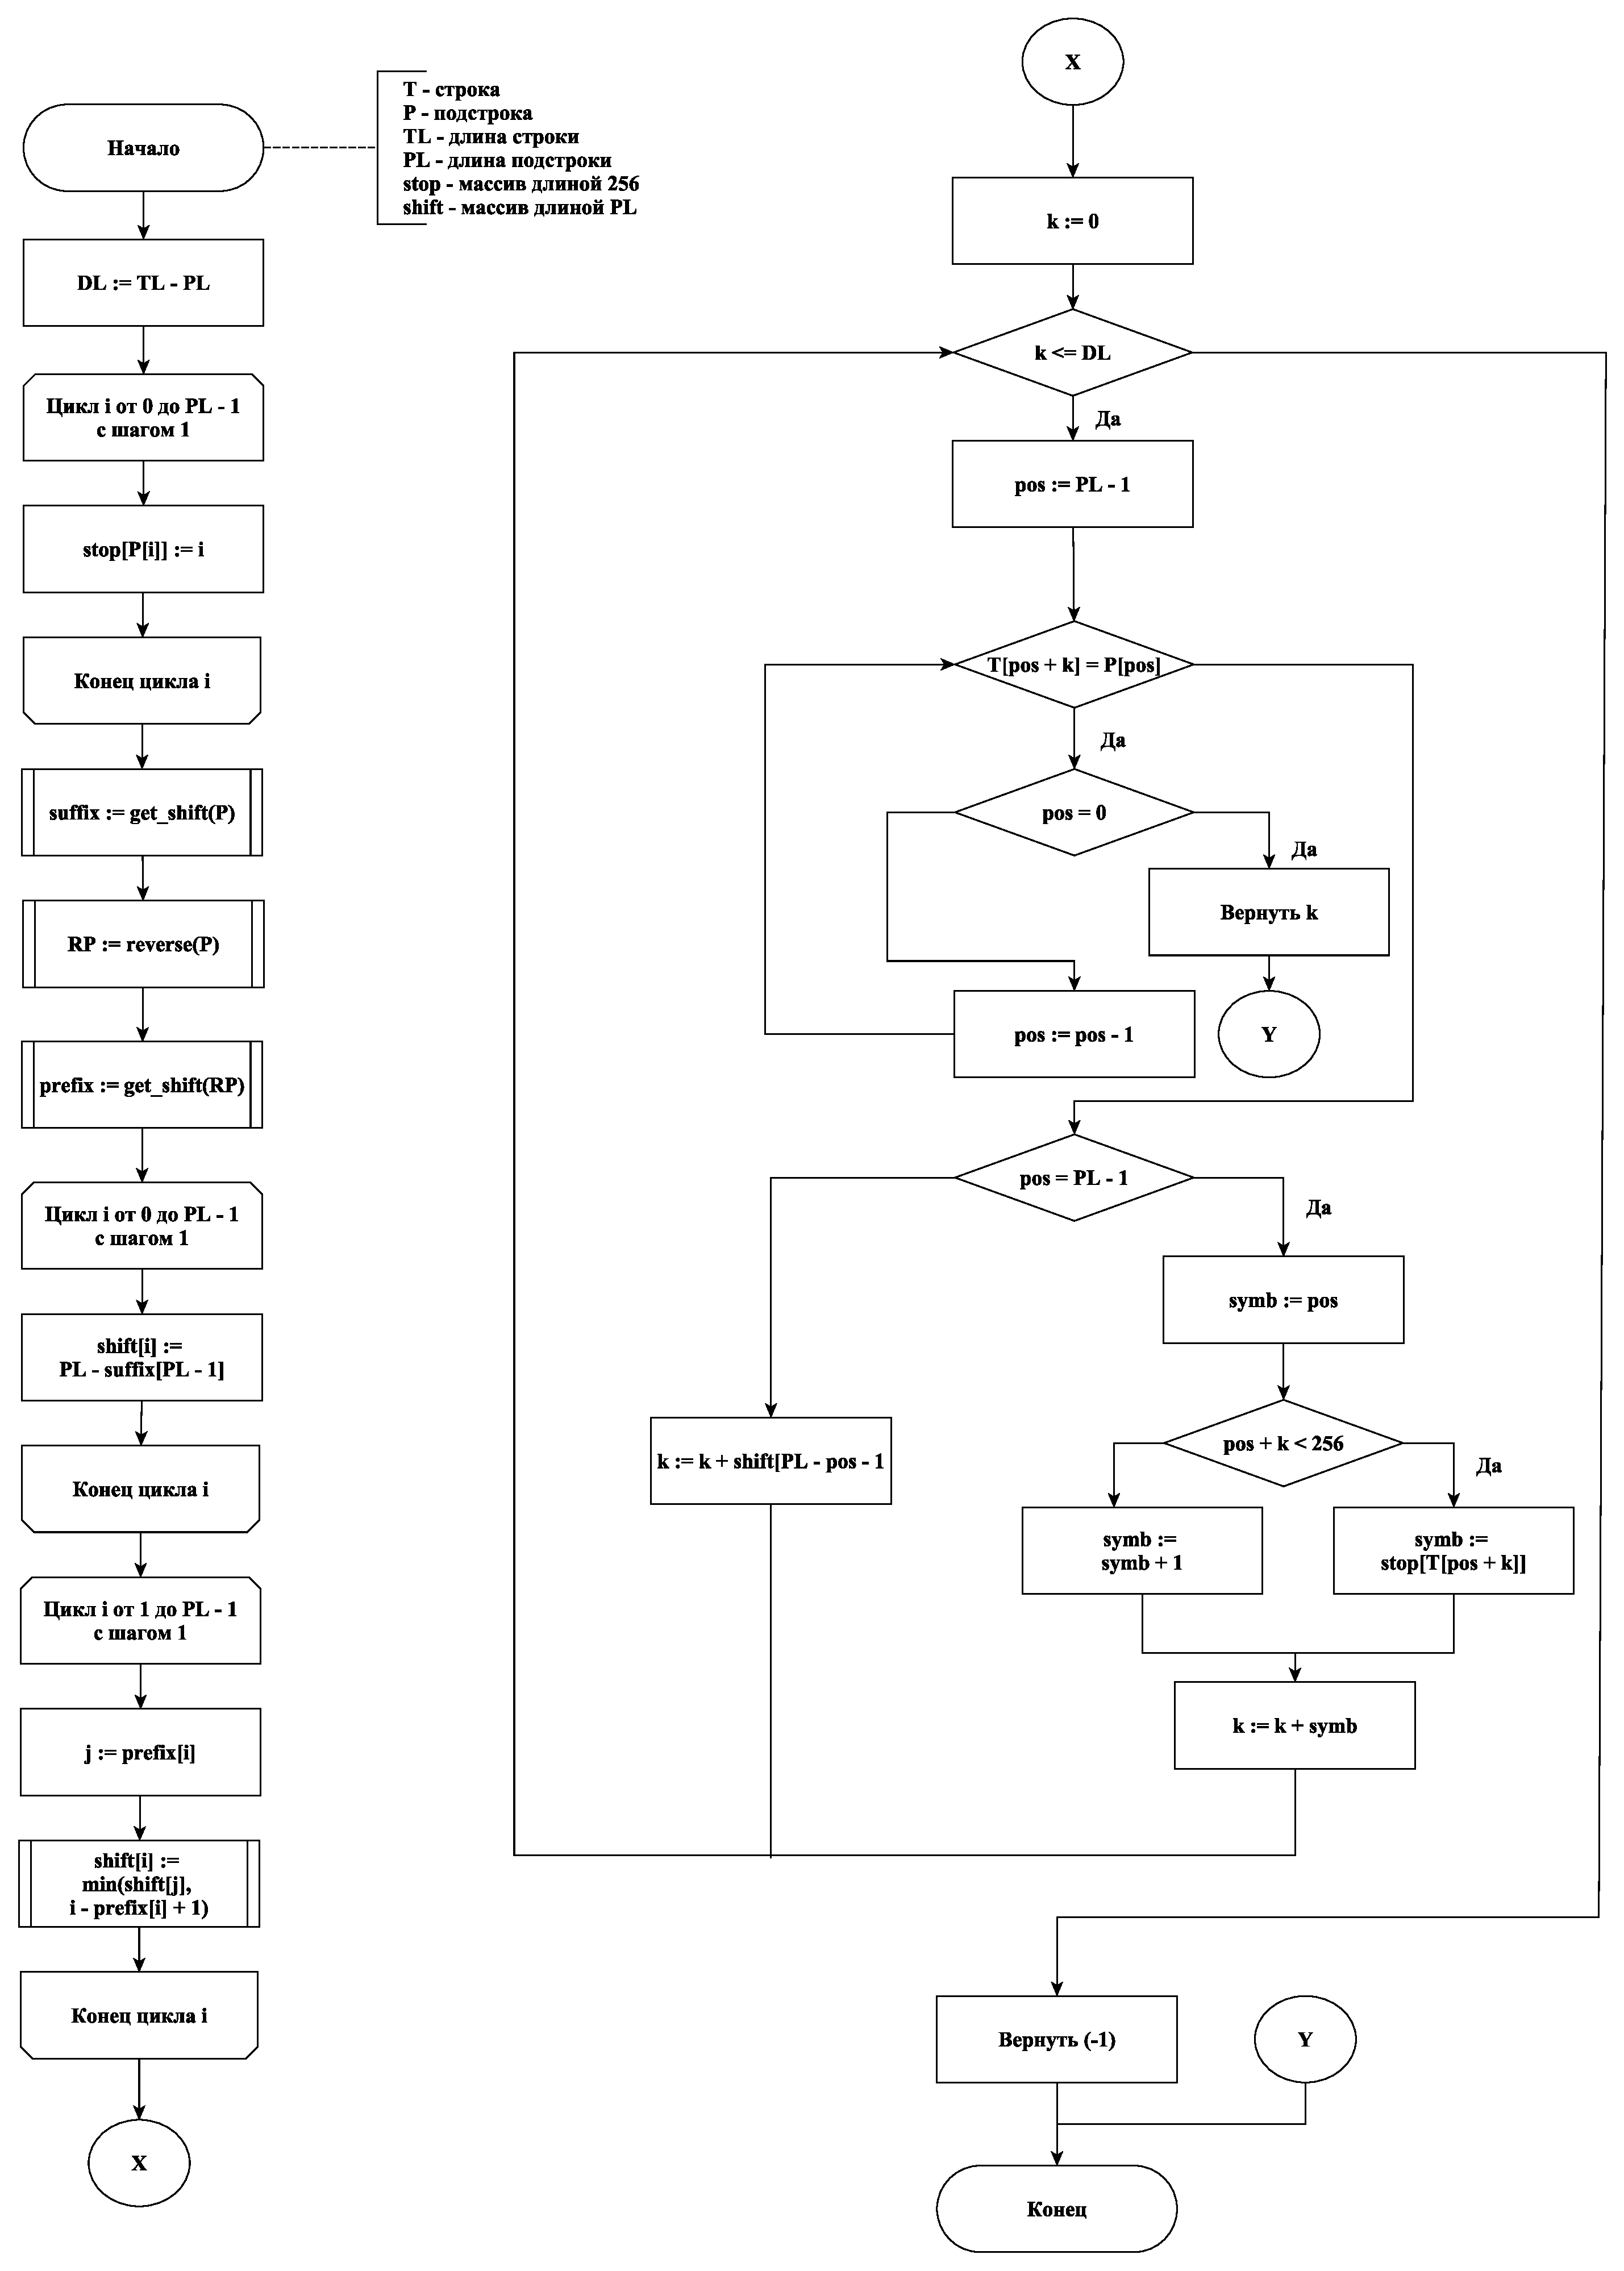
\includegraphics[scale = 0.35]{diagram/bm.pdf}}
\caption{
Схема алгоритма Бойера-Мура}
\label{fig:bm}
\end{center}
\end{figure}

\pagebreak

\subsection{Сравнительный анализ алгоритмов}
\label{fig:cmp_section}

\subsubsection{Пример работы алгоритма Кнута-Морриса-Пратта}

Рассмотрим пример работы алгоритмов на
строке \textit{ababqcabababakababacqw} длиной 22 символа
и подстроке \textit{ababac} длиной 6 символов.

Сперва необходимо построить префикс-функцию для подстроки. Для этого
последовательно пройдем по подстроке в поисках очередного максимального суффикса,
равного префиксу. Пошаговый разбор представлен в таблице \ref{pref}:
слева отмечен индекс нового входящего символа, посередине ---
рассматриваемая строка, справа --- значение префикс-функции.
\textit{Курсивом} и \textbf{жирным} выделены совпадающие максимальные
\textit{префиксы} и \textbf{суффиксы}.

\begin{table} [h!]
\begin{center}
\caption{Нахождение префикс-функции}
\begin{tabular}{|r|rrrrrr|r|}
\hline
Индекс & Строка & & & & & & Префикс-функция \\
\hline
         0 &          a &            &            &            &            &            &          0 \\

         1 &          a &          b &            &            &            &            &          0 \\

         2 &    {\it a} &          b &    {\bf a} &            &            &            &          1 \\

         3 &    {\it a} &    {\it b} &    {\bf a} &    {\bf b} &            &            &          2 \\

         4 &    {\it a} &    {\it b} & {\bfseries {\itshape a}} &    {\bf b} &    {\bf a} &            &          3 \\

         5 &          a &          b &          a &          b &          a &          c &          0 \\
\hline
\end{tabular}
\label{pref}
\end{center}
\end{table}  

Далее уже применим похожий подход для поиска подстроки.
При несовпадении символов, будем смещать подстроку таким образом, чтобы 
префикс строки (до нового рассматриваемого символа этой строки) был равен
некоторому префиксу подстроки (табл. \ref{kmp_cmp}).

\begin{table} [h!]
\begin{center}
\caption{Пример работы алгоритма Кнута-Морриса-Пратта}
\begin{tabular}{|rrrrrrrrrrrrrrrrrrrrrrr|}
\hline
           &          0 &          1 &          2 &          3 &          4 &          5 &          6 &          7 &          8 &          9 &         10 &         11 &         12 &         13 &         14 &         15 &         16 &         17 &         18 &         19 &         20 &         21 \\

           &          a &          b &          a &          b &    {\bf q} &    {\bf c} &          a &          b &          a &          b &          a &    {\bf b} &          a &    {\bf k} &          a &          b &          a &          b &          a &          c &          q &          w \\

         1 &    {\bf a} &    {\bf b} &    {\bf a} &    {\bf b} &    {\bf a} &          c &            &            &            &            &            &            &            &            &            &            &            &            &            &            &            &            \\

         2 &            &            &            &            &            &    {\bf a} &          b &          a &          b &          a &          c &            &            &            &            &            &            &            &            &            &            &            \\

         3 &            &            &            &            &            &            &    {\bf a} &    {\bf b} &    {\bf a} &    {\bf b} &    {\bf a} &    {\bf c} &            &            &            &            &            &            &            &            &            &            \\

         4 &            &            &            &            &            &            &            &            &    {\bf a} &    {\bf b} &    {\bf a} &    {\bf b} &    {\bf a} &    {\bf c} &            &            &            &            &            &            &            &            \\

         5 &            &            &            &            &            &            &            &            &            &            &            &            &            &            &    {\bf a} &    {\bf b} &    {\bf a} &    {\bf b} &    {\bf a} &    {\bf c} &            &            \\
\hline
\end{tabular}  
\label{kmp_cmp}
\end{center}
\end{table}

\begin{itemize}
\item[1)] несовпадение происходит на символе с индексом 4,
подходящего префикса нет, поэтому следующее сравнение начинаем с 5 символа;
\item[2)] аналогичная ситуация;
\item[3)] несовпадение на 11 символе, суффикс \textit{abab}
равен префиксу подстроки, значение префикс-функции для данной части подстроки
равно 2, поэтому смещаем подстроку на 2 символа вправо;
\item[4)] аналогичный случай в 1-2 этапах;
\item[5)] полное совпадение.
\end{itemize}

Для нахождения потребовалось 5 сравнений на первом этапе, 1 --- на втором,
по 6 --- на остальных этапах. Итого, 24 сравнения. В наивном алгоритме
потребовалось бы 38 сравнений.

\subsubsection{Пример работы алгоритма Бойера-Мура}

Рассмотрим работу алгоритм Бойера-Мура на тех же входных данных.

В алгоритме Бойера-Мура необходимо дополнительно найти
массив стоп-символов и массив сдвигов.
Длина массива стоп-символов равна мощности алфавита, над которым производятся действия.
Для каждого уникального символа подстроки вычислим индекс самого последнего вхождения
и занесем его в этот массив, для остальных символов поставим значение равное -1.
Итак, для \textit{a} -- 4, \textit{b} -- 3, \textit{c} -- 5.

Для каждого возможного суффикса шаблона указываем наименьшую величину,
на которую нужно сдвинуть вправо шаблон,
чтобы он снова совпал с префиксом и при этом символ,
предшествующий этому вхождению, не совпадал бы с символом, предшествующим суффиксу.
Если такой сдвиг невозможен, ставится длина подстроки (табл. \ref{shift_}).

\begin{table} [h!]
\begin{center}
\caption{Массив сдвигов в алгоритме Бойера-Мура}
\begin{tabular}{|r|rrrrrr|}
\hline
Индекс & 0 &          1 &          2 &          3 &          4 &          5 \\
\hline
Строка &         a &          b &          a &          b &          a &          c \\
\hline
Сдвиг &         6 &          2 &          3 &          4 &          5 &          6 \\
\hline
\end{tabular}  
\label{shift_}
\end{center}
\end{table}

Теперь можно перейти непосредственно к поиску подстроки (табл. \ref{bm_cmp}).

\begin{table} [h!]
\begin{center}
\caption{Пример работы алгоритма Бойера-Мура}
\begin{tabular}{|rrrrrrrrrrrrrrrrrrrrrrr|}
\hline
           &          0 &          1 &          2 &          3 &          4 &          5 &          6 &          7 &          8 &          9 &         10 &         11 &         12 &         13 &         14 &         15 &         16 &         17 &         18 &         19 &         20 &         21 \\

           &          a &          b &          a &          b &    {\bf q} &          c &          a &    {\bf b} &          a &    {\bf b} &          a &    {\bf b} &          a &    {\bf k} &          a &          b &          a &          b &          a &          c &          q &          w \\

         1 &          a &          b &          a &          b &    {\bf a} &    {\bf c} &            &            &            &            &            &            &            &            &            &            &            &            &            &            &            &            \\

         2 &            &            &          a &          b &          a &          b &          a &    {\bf c} &            &            &            &            &            &            &            &            &            &            &            &            &            &            \\

         3 &            &            &            &            &          a &          b &          a &          b &          a &    {\bf c} &            &            &            &            &            &            &            &            &            &            &            &            \\

         4 &            &            &            &            &            &            &          a &          b &          a &          b &          a &    {\bf c} &            &            &            &            &            &            &            &            &            &            \\

         5 &            &            &            &            &            &            &            &            &          a &          b &          a &          b &          a &    {\bf c} &            &            &            &            &            &            &            &            \\

         6 &            &            &            &            &            &            &            &            &            &            &            &            &            &            &    {\bf a} &    {\bf b} &    {\bf a} &    {\bf b} &    {\bf a} &    {\bf c} &            &            \\
\hline
\end{tabular}  
\label{bm_cmp}
\end{center}
\end{table}

\begin{itemize}
\item[1)] несовпадение происходит на символе с индексом 4,
префикс \textit{ab} совпадает с суффиксом, поэтому смещаемся на 2
в соответствии с массивом сдвигов;
\item[2-5)] аналогичная ситуация несовпадения,
только смещение происходит по стоп-таблице, так как нет подходящего суффикса;
\item[6)] полное совпадение.
\end{itemize}

Для нахождения потребовалось 2 сравнения на первом этапе,
4 --- на последнем этапе, по 1 --- на всех остальных. Всего 12 сравнений.

\subsubsection{Оценка времени работы алгоритма Кнута-Морриса-Пратта}

Рассмотрим сравнение строк на позиции
$i$, где образец $S[0, m - 1]$
сопоставляется с частью текста
$T[i, i + m - 1]$.
Предположим, что первое несовпадение произошло
между $T[i + j]$ и $S[j]$,
где $1 < j < m$. Тогда
$T[i, i + j - 1] = S[0, j - 1] = P$ и
$a = T[i + j] \neq S[j] = b$.

При сдвиге вполне можно ожидать, что префикс 
(начальные символы)
образца $S$ сойдется с каким-нибудь суффиксом 
(конечные символы) текста $P$. Длина наиболее 
длинного префикса, являющегося одновременно 
суффиксом, есть значение префикс-функции от строки 
$S$ для 
индекса $j$.

Это приводит нас к следующему алгоритму: пусть
$\pi[j]$ -- значение префикс-функции от 
строки $S[0, m - 1]$ для индекса $j$. 
Тогда после сдвига мы можем возобновить сравнения с 
места $T[i + j]$ и $S[\pi[j]]$ без потери возможного 
местонахождения образца. Можно показать, 
что таблица 
сдвигов может быть вычислена
за $\mathbf{O(m)}$ сравнений перед 
началом поиска. А поскольку строка $T$ будет 
пройдена 
ровно один раз, суммарное время работы алгоритма 
будет равно $\mathbf{O(m + n)}$, где $n$ -- длина 
текста $T$. ~\cite{knuth}

\subsubsection{Оценка времени работы алгоритма Бойера-Мура}

Ниже мы обозначаем через $\mathbf{A}$ — число символов в алфавите.

При подсчете массива сдвигов по одному присваиванию приходится
на каждый элемент массива и еще по одному -- на каждый символ
образца. Поэтому общее число присваиваний равно $\mathbf{O(m + A)}$.
При вычислении массива прыжков в худшем случае каждый символ
образца будет сравниваться со всеми последующими его символами.

Можно подсчитать, что число сравнений в худшем случае
будет $\mathbf{O(mn)}$. В лучшем случае асимптотика равна $\mathbf{O(m + n)}$.
~\cite{eng_bm}


\subsection*{Выводы}
\addcontentsline{toc}{subsection}{Выводы}

В разделе представлены схемы алгоритмов поиска подстроки в строке
Кнута-Морриса-Пратта и Бойера-Мура.
Произведен теоретический анализ
временной сложности, обозначены различия в работе алгоритмов,
пояснена их эффективность.
\newpage
\section{Технологический раздел}

В данном разделе описываются требования к программному 
обеспечению и средства реализации, приводятся листинги 
программы и тестовые данные.

\subsection{Требования к программному обеспечению}

\begin{flushleft}
\textbf{Входные данные:} 
\begin{itemize}
\item \textit{text} --- строка, в которой ведется поиск;
\item \textit{pattern} --- искомая подстрока.
\end{itemize}
	
\textbf{Выходные данные:} индекс первого вхождения
подстроки \textit{pattern} в строке
\textit{text}; при отсутствии подстроки либо неверных данных
(длина подстроки превышает длину строки) --- сообщение об ошибке.
\end{flushleft}
	
На рис. \ref{fig:idef0} приведена 
функциональная схема 
программы поиска подстроки в строке.
        
\begin{figure}[h!]
\begin{center}
{\includegraphics[width = \textwidth]{img/idef0.png}}
\caption{Функциональная схема 
программы поиска подстроки в строке}
\label{fig:idef0}
\end{center}
\end{figure}
	
\newpage
\subsection{Средства реализации}

Программа написана на языке С++, т. к. этот язык предоставляет программисту широкие возможности реализации самых разнообразных алгоритмов, обладает высокой эффективностью и значительным набором стандартных классов и процедур. В качестве среды разработки использовался  фреймворк QT 5.13.1.
	
	Для хранения массивов и строк были использованы стандартные контейнерные классы std::vector и std::vector соответственно.
	
	Для замера времени выполнения программы использовалась библиотека chrono.
	
    
\subsection{Листинг программы}

В листингах  \ref{lst0}, \ref{lst1} и \ref{lst2} представлены реализации алгоритмов Кнута-Морриса-Пратта и Бойера-Мура .

\begin{lstlisting}[label=lst0,caption=Реализация
заполнения массива сдвигов]
std::vector<int> get_shift(const std::string &str) {
    int len = str.length();
    std::vector<int> shift(len, 0);

    for (int i = 1, j = 0; i < len; ++i) {
        while (j > 0 && str[i] != str[j]) {
            j = shift[j - 1];
        }

        if (str[i] == str[j]) {
            ++j;
        }

        shift[i] = j;
    }

    return shift;
}
\end{lstlisting}

\begin{lstlisting}[label=lst1,caption=Реализация
алгоритма Кнута-Морриса-Пратта]
int kmp_search(const std::string &text, const std::string &pattern) {
    if (text.length() < pattern.length()) {
        return WRONG_LEN;
    }

    const int text_len = text.length();
    const int pattern_len = pattern.length();

    auto shift = get_shift(pattern);

    for (int i = 0, j = 0; i < text_len; ++i) {
        while (j > 0 && text[i] != pattern[j]) {
            j = shift[j - 1];
        }

        if (text[i] == pattern[j]) {
            ++j;
        }

        if (pattern_len == j) {
            return i - pattern_len + 1;
        }
    }

    return NOT_FOUND;
}
\end{lstlisting}

\begin{lstlisting}[label=lst2,caption=Реализация
алгоритма Бойера-Мура]
int bm_search(const std::string &text, const std::string &pattern) {
    if (text.length() < pattern.length()) {
        return WRONG_LEN;
    }

    const int text_len = text.length();
    const int pattern_len = pattern.length();
    const int dif_len = text_len - pattern_len;

    const int ascii_num = 256;
    std::vector<int> stop_table(ascii_num, -1);
    std::vector<int> shift_table(pattern_len);

    for (int i = 0; i < pattern_len; ++i) {
        stop_table[pattern[i]] = i;
    }

    std::string rev_pattern(pattern.rbegin(), pattern.rend());
    auto suffix_table = get_shift(pattern);
    auto prefix_table = get_shift(rev_pattern);

    for (int i = 0; i < pattern_len + 1; ++i) {
        shift_table[i] = pattern_len - suffix_table.back();
    }

    for (int i = 1; i < pattern_len; ++i) {
        int j = prefix_table[i];
        shift_table[i] = std::min(shift_table[j], i - prefix_table[i] + 1);
    }

    int shift = 0;
    while (shift <= dif_len) {
        int pos = pattern_len - 1;

        while (text[pos + shift] == pattern[pos]) {
            if (0 == pos) {
                return shift;
            }

            --pos;
        }

        if (pattern_len - 1 == pos) {
            int stop_symb = pos;

            if (pos + shift < ascii_num) {
                stop_symb -= stop_table[text[pos + shift]];
            } else {
               ++stop_symb;
            }

            shift += stop_symb;
        } else {
            shift += shift_table[pattern_len - pos - 1];
        }
    }

    return NOT_FOUND;
}
\end{lstlisting}

\subsection{Тестовые данные}
\label{fig:test_data}

Программа должна корректно выполнять поиск подстроки в строке при входных данных, приведенных в таблице \ref{test0}.

\begin{table} [h!]
\begin{center}
\caption{Тестовые данные}
\begin{tabular}{|r|r|r|r|}
\hline
         № &     Строка &  Подстрока &  Результат \\
\hline
         1 &          a &        abc &  $\text{Неверная длина}$ \\
\hline
         2 &        abc &       abcd &  $\text{Неверная длина}$ \\
\hline
         3 &        abc &        def &  $\text{Не найдено}$ \\
\hline
         4 &        abc &         aa &  $\text{Не найдено}$ \\
\hline
         5 &  abbaabbab &       aaab &  $\text{Не найдено}$ \\
\hline
         6 &        abc &          a &          0 \\
\hline
         7 &  abbaabbab &       abba &          0 \\
\hline
         8 &        abc &          b &          1 \\
\hline
         9 &  abbaabbab &       baab &          2 \\
\hline
        10 & there they are &       they &          6 \\
\hline
        11 &        abc &          c &          2 \\
\hline
        12 &  abbaabbab &       bbab &          5 \\
\hline
        13 & there they are &        are &         11 \\
\hline
        14 &     abcabc &          a &          0 \\
\hline
        15 &     abcabc &          c &          2 \\
\hline
        16 & abbaabbabbbab &       bbab &          5 \\
\hline
        17 & there they are are here are &        are &         11 \\
\hline
        18 &          a &          a &          0 \\
\hline
        19 &        abc &        abc &          0 \\
\hline
        20 & abbaabbabbbab & abbaabbabbbab &          0 \\
\hline
\end{tabular} 

\label{test0}
\end{center}
\end{table}

\subsection*{Выводы}
\addcontentsline{toc}{subsection}{Выводы}

В данном разделе были рассмотрены требования к 
программному обеспечению, обоснован выбор средств 
реализации, приведены листинги программы и тестовые 
данные.

\newpage
\section{Исследовательский раздел}

В разделе представлены примеры выполнения программы,
а также результаты исследования эффективности сортировок.

\subsection{Примеры работы}
        
На рис. \ref{fig:t0}-\ref{fig:t6} приведены примеры работы программы. 
        
\begin{figure}[h!]
\center{\includegraphics[scale = 0.8]{img/0.png}}
\caption{
Пустой ввод}
\label{fig:t0}
\end{figure}

\begin{figure}[h!]
\center{\includegraphics[scale = 0.8]{img/1.png}}
\caption{
Некорректная длина строки}
\label{fig:t1}
\end{figure}

\begin{figure}[h!]
\center{\includegraphics[scale = 0.8]{img/2.png}}
\caption{
Подстрока не найдена}
\label{fig:t2}
\end{figure}

\pagebreak

\begin{figure}[h!]
\center{\includegraphics[scale = 0.8]{img/3.png}}
\caption{
Подстрока в начале}
\label{fig:t3}
\end{figure}

\begin{figure}[h!]
\center{\includegraphics[scale = 0.8]{img/4.png}}
\caption{
Подстрока в середине}
\label{fig:t4}
\end{figure}

\begin{figure}[h!]
\center{\includegraphics[scale = 0.8]{img/5.png}}
\caption{
Подстрока в конце}
\label{fig:t5}
\end{figure}

\begin{figure}[h!]
\center{\includegraphics[scale = 0.8]{img/6.png}}
\caption{
Повтор подстроки}
\label{fig:t6}
\end{figure}

\pagebreak


\subsection{Постановка эксперимента}
    
Необходимо cравнить время работы алгоритмов Кнута-Морриса-Пратта и Бойера-Мура.  Замеры произвести на строках длиной от 100 тыс. до 1 млн. символов с шагом 100 тыс. символов, длина искомой подстроки -- 100 символов, каждый замер выполняется 1000 раз.
Строка содержит только символы \textit{a},
в подстроке символы \textit{b} и \textit{a}
чередуются (реализуется худший случай для
алгоритма Бойера-Мура).

\subsection{Сравнительный анализ на основе эксперимента}

Замеры производились на компьютере следующей конфигурации: 
\begin{enumerate}
\item[1)] процессор: Intel Core i5 1.8 ГГц, 8 логических ядер; 
\item[2)] ОЗУ: 8 Гб, 2400 МГц DDR4;
\item[3)] ОС: Windows 10.
\end{enumerate}

На рис. \ref{fig:chart_substr} приводятся графики сравнения времени выполнения алгоритмов.

\begin{figure}[h!]
\center{
\includegraphics[width = \textwidth]{chart/chart_substr.pdf}}
\caption{Сравнение времени выполнения алгоритмов поиска подстроки в строке}
\label{fig:chart_substr}
\end{figure}

Как видно, подтверждены теоретические расчеты. В худшем случае
асимптотика алгоритма Бойера-Мура квадратична, а Кнута-Морриса-Пратта -- линейна.

\subsection*{Выводы}
\addcontentsline{toc}{subsection}{Выводы}

Программа успешно прошла все заявленные тесты. Эксперименты замера времени подтвердили предположения и
теоретические расчеты из раздела \ref{fig:cmp_section}.

\newpage
\section*{Заключение}
\addcontentsline{toc}{section}{Заключение}

В ходе работы выполнено следующее:
	
\begin{enumerate} 
\item[1)] изучены алгоритмы поиска подстроки в строке;
\item[2)] применен метод динамического программирования для  
реализации указанных алгоритмов;
\item[3)] проведен сравнительный анализ алгоритмов по времени выполнения;
\item[4)] экспериментально подтверждены различия во временнóй эффективности алгоритмов 
при помощи разработанного программного обеспечения на материале замеров процессорного 
времени на строках различных размеров; в худшем случае
асимптотика алгоритма Бойера-Мура квадратична, а Кнута-Морриса-Пратта -- линейна;
\item[5)] описаны и обоснованы полученные результаты в отчете о лабораторной 
работе, выполненного как расчётно-пояснительная записка. 
\end{enumerate}

\newpage
\addcontentsline{toc}{section}{Список литературы}
\begin{thebibliography}{8}

\bibitem{mcconell}
Дж. Макконнелл. Анализ алгоритмов. Активный 
обучающий 
подход.-М.:Техносфера, 2009.

\bibitem{knuth}
Д. Кнут. Искусство программирования, М., Мир, 1978

\bibitem{search}
Алгоритмы поиска в строке [Электронный ресурс]. – Режим доступа: https://habr.com/ru/post/111449//, свободный – (26.11.2019)

\bibitem{kmp_}
Поиск подстроки. Алгоритм Кнута–Морриса-Пратта [Электронный ресурс]. – Режим доступа: https://habr.com/ru/post/191454/, свободный – (21.11.2019)

\bibitem{bminfo}
Алгоритм Бойера-Мура для поиска по шаблону [Электронный ресурс]. – Режим доступа: http://espressocode.top/boyer-moore-algorithm-for-pattern-searching/, свободный – (26.11.2019)

\bibitem{eng_bm}
Алгоритм Бойера-Мура для поиска по шаблону [Электронный ресурс]. – Режим доступа: http://www-igm.univ-mlv.fr/~lecroq/string/node14.html, свободный – (26.11.2019)

\bibitem{std}
ISO/IEC 14882:2017 [Электронный ресурс]. – Режим доступа: https://www.iso.org/standard/68564.html, свободный – (27.11.2019)

\bibitem{chrono}
<chrono> [Электронный ресурс]. – Режим доступа: http://www.cplusplus.com/reference/chrono/, свободный – (20.11.2019)

\end{thebibliography}


\end{document}
